\lecture{13}{thu 13 oct 11:00}{Calculating}
\section{Calculating Price Elasticity of Demand}
To calculate the price elasticity, you have two options. There is the percent change formula and the total revenue test. You should only use the total revenue test if the percent change info is not given. The rest of the time you should be using the percent change formula when you have percents. 
\begin{definition}
    \[
        E_D = \frac{\%\Delta QD}{\%\Delta\text{Price}}
    .\] 
\end{definition}

Lets say that Quantity falls by 15\% and as a result, Price rises by 10\%, you just have to do:
\[
    E_D  = \frac{15\%}{10\%} = 1.5
.\] 

Since the $E_D$ is greater than 1, the demand is elastic. This is where those definitions that were mentioned earlier come in handy, but as a refreshers, if $E_D$ is equal to 1, its unit. Otherwise if its greater than 1 its elastic, and less than 1 if its inelastic. I wanna emphasize a point, that even if the slope of the line is constant, the elasticity is not. Make sure to actually do the calculations to find the elasticity.

Now you should also know how to calculate percent change, which is commonly, 
 \[
     \%\Delta = \frac{\text{new-old}}{\text{old}} * 100\%
.\] 

Since P and Q move in opposite directions on a demand curve, it is common to get a negative price elasticity and drop the negative sign. Lets try an example with a graph. 

\begin{figure}[h!]
\begin{center}
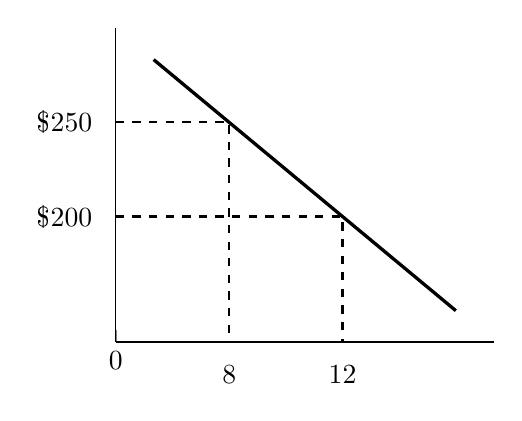
\begin{tikzpicture}
\begin{axis}[
scale=0.7,
xmin = 0, xmax = 10,
ymin = 0, ymax = 10, 
axis lines* = left,
xtick = {0}, ytick = \empty,
axis on top, 
clip = false,
]

\addplot[color = black, very thick] coordinates {(1,9) (9,1)};
\addplot[color = black, dashed, thick] coordinates {(0,7) (3,7) (3,0)};
\addplot[color = black, dashed, thick] coordinates {(0,4) (6,4) (6,0)};

\node[left = 5pt] at (0,7) {\$250};
\node[left = 5pt] at (0,4) {\$200};
\node[below = 5pt] at (3,0) {8};
\node[below = 5pt] at (6,0) {12};
\end{axis}
\end{tikzpicture}
\end{center}
\end{figure}

Lets calculate from \$250 to \$200,
\[
    \%\Delta = \frac{200-250}{250} = -0.2
.\] 

Add since we did a falling price, we need to calculate a increasing QD,
\[
    \%\Delta = \frac{12-8}{8} = 0.5
.\] 

Then we can just plug those values into the equation, 
\[
    E_D = \frac{50}{20} = 2.50
.\] 

Since $E_D$ is greater than 1, the graph is elastic. However there is a flaw with the percent change method. If done with price as a increase, you actually get a elasticity of 1.33. Still greater than 1, but be careful to make sure you are doing the correct percent changes. 

Now there is a midpoint method, and in my opinion, it is much easier,
 \[
     E_D = \frac{\frac{(Q_2-Q_1)}{\frac{Q_2+Q_1}{2}}}{\frac{(P_2-P_1)}{\frac{P_2+P_1}{2}}}
.\] 
It doesnt matter what value is chosen, as long as they are consistent throughout the formula. However at the current moment I dont recommend using this formula, as it is outputting different values compared to the percent change formula. Since the AP exam focuses more on percent change, thats what I recommend for now. 

Now there is a different way to calculating this which I mentioned earlier. The \textbf{Total Revenue Test} is a way of just measuring profit, and how elasticity can affect it. This will not net you a number with the elasticity, but it is a good way of visually comparing. 

Well what is total revenue? Good question, total revenue is simply, 
\[
TR = P * Q
.\] 

I am not going to cover why this is in too much detail, since it is basic algebra. All you have to do then is just compare the starting price and the total revenue. If price and total revenue move in the same directionm it is inelastic, and the opposite results in elastic.

Now there are some really specific things like price effect and stuff that shows how this works, but I am not going to include them. You can look them up if you want to learn more, but they really dont provide much for understanding. 
